\documentclass[12pt]{article}

\usepackage{sbc-template}
\usepackage{graphicx,url}
\usepackage{amsmath}
\usepackage[utf8]{inputenc}
\usepackage[T1]{fontenc}

\sloppy

\title{Efficient Computation of the Directional Extremal Boundary\\of a Union of Equal-Radius Circles}

\author{Juliana Almeida\inst{1}}

\address{Instituto de Computação (IComp) -- Universidade Federal do Amazonas (UFAM)\\
  Manaus -- AM -- Brasil\\
  \email{juliana.almeida@icomp.ufam.edu.br}
}

\begin{document}

\maketitle

\begin{abstract}
This paper focuses on computing the directional extremal boundary
of a union of equal-radius circles. We introduce an efficient algorithm
that accurately determines this boundary by analyzing the intersections and
dominant relationships among the circles. The algorithm has time complexity
of $O(n \log n)$.
\end{abstract}

\section{Introduction}

Computing the directional extremal boundary of a union of equal-radius circles involves
identifying the outermost points in a specified direction that form the outer edge of the
combined circle regions. This task is essential in a wide range of applications where each
circle may represent a measurement, area of influence, or coverage zone.

Without loss of generality, this paper focuses on computing the upper boundary of
the union of unit circles, as this can be readily extended to circles of any equal radius by
applying uniform scaling and rotation. In this paper, we present an efficient algorithm for
determining the upper boundary of overlapping unit circles. The method begins by sorting
all circle centers according to their horizontal positions. Once sorted, the circles are
processed from left to right to build the boundary incrementally, accounting for overlaps
and overshadowing. Specifically, it identifies the exact horizontal positions where one
circle's boundary overtakes or merges into another's. By maintaining a dynamic list of
circles that currently define the boundary, the algorithm eliminates any circles that no
longer contribute to the highest points, thereby preserving only those that shape the overall
upper boundary.

One practical application of this algorithm is the precise localization of extremal
points along elongated structures such as rail tracks or pipelines. In such cases, each
circle may represent a measurement along the structure, and computing the circles'
directional extremal boundary enables accurate identification of the outermost positions
in the specified direction.

Another application arises in robotic workspace modeling, where a robotic arm
moves along rails in one direction and extends in another. Here, circles can represent
obstacles and safety zones: the circle centers reflect object positions, while radii model
object sizes, arm dimensions, and required safety distances. The algorithm can then
determine safe regions in which the arm may operate without collisions.

\section{Problem Statement}

Given $n$ unit circles $C_i$ centered at $\mathbf{c}_i = (x_i, y_i)$ for $i = \overline{1,n}$,
our objective is to compute the maximum envelope function $f(x)$ representing the upper
boundary of their union:

\[
f(x) = \max_{|x - x_i| \leq 1,\; i \in \overline{1,n}} \left( y_i + \sqrt{1 - (x - x_i)^2} \right).
\]

This function identifies the highest point among the circles at any horizontal position $x$,
as illustrated in Figure~\ref{fig:upper_boundary}.

\begin{figure}[ht]
\centering
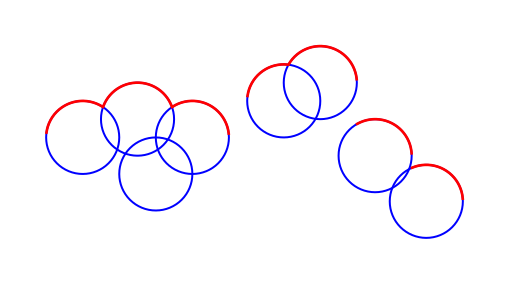
\includegraphics[width=0.6\textwidth]{example_with_unused_and_lower_circle.png}
\caption{Visualization of the upper boundary of unit circles. The circles are
shown as blue and red arcs, with the red arcs forming the upper boundary,
which defines the highest points along the $y$-axis.}
\label{fig:upper_boundary}
\end{figure}

Circles whose centers are separated by a horizontal distance of at least twice the
radius (i.e., two units for unit circles) do not intersect and can be processed independently.
Furthermore, if multiple circles have the same horizontal coordinate $x_i$, only the circle
with the highest vertical coordinate $y_i$ contributes to the upper boundary.

\section{Algorithm Description}

The algorithm constructs the upper boundary by iteratively processing the circles. The
resultant upper boundary is a piecewise curve composed of circular arcs. We group
these arcs into \textit{segments}, where each segment is a horizontally continuous portion of
the boundary. In other words, the upper boundary can be viewed as an ordered list of
segments, with each segment separated horizontally.

Within each segment, the arcs are determined by the relationships between
consecutive circles. To handle these relationships efficiently, the algorithm maintains a
sequence of circles along with their corresponding horizontal transition positions. This
sequence defines a single segment of the boundary. As the algorithm proceeds, it finalizes
segments whenever it encounters a horizontal gap and then starts a new segment. To
summarize, there are three cases for how the arcs form the boundary (two of which cause
discontinuities---gaps and overshadowing):

\begin{itemize}
    \item When arcs are directly connected, meaning one arc ends where the next begins
    without any gap
    \item When one circle overshadows another within the same horizontal span, defining
    the upper boundary without introducing a horizontal gap, while the arcs remain in
    the same segment
    \item When the arcs are horizontally separated and therefore form distinct segments
\end{itemize}

The algorithm consists of the following steps:

\begin{enumerate}
    \item Sort the circles in ascending order based on their $x_i$ coordinates.
    \item For each unique $x_i$ coordinate, retain only the circle with the highest $y_i$ coordinate
    and discard the others.
    \item Initialize an empty list of segments.
    \item Iterate through each circle $C_i$ in the sorted list:
    \begin{enumerate}
        \item If there are no segments, create a new segment, add $C_i$ to it, and proceed
        to the next circle.
        \item Determine the horizontal transition position between the last circle, $C_j$, in
        the last segment and $C_i$ using the method described in Section~\ref{sec:appendix}.
        \item If the circles do not overlap (i.e., there is a horizontal gap), then create a
        new segment, add $C_i$ to it, and proceed to the next circle.
        \item If the current segment has horizontal transition positions and the last
        horizontal transition position is more than or equal to the computed
        horizontal transition position $x_u$:
        \begin{enumerate}
            \item Remove $C_j$ and the last horizontal transition position from the
            current segment. Set $C_j$ to be the circle currently at the end of
            the segment.
            \item Recompute the transition position between the segment's new last
            circle, $C_j$, and $C_i$. If no intersection is found (which can happen
            due to floating-point roundoff errors), use the midpoint of their
            centers' $x$ coordinates as the transition position.
            \item Repeat step 4(d).
        \end{enumerate}
        \item Otherwise, add the horizontal transition position $x_u$ and $C_i$ to the current
        segment.
    \end{enumerate}
\end{enumerate}

\section{Proof of Algorithm Correctness}

\subsection*{Uniqueness of Horizontal Transition}

\textbf{Lemma 1:} For any two unit circles $C_j$ and $C_i$ with centers $\mathbf{c}_j = (x_j, y_j)$ and
$\mathbf{c}_i = (x_i, y_i)$ such that $x_j < x_i$ and $x_i - x_j < 2$, there exists only one horizontal
position $x_u$ where the upper extremal boundaries of the circles transition from one circle to the other.

\textbf{Proof of Lemma 1:}

For each unit circle, we only need to consider the upper half of the circle as it
shadows the lower half. There are two cases to consider: when the upper halves of the
unit circles intersect and when they do not intersect.

First, consider the case where the upper halves intersect. They can have at most
one intersection point $x_u$. Suppose, for the sake of contradiction, that there are multiple
intersection points. Due to symmetry about the midpoint between the centers of the
circles, there would also be multiple intersections between the lower halves of the circles.
This would result in more than two intersection points between the circles overall, which
is impossible for circles. Therefore, only one intersection between the upper halves is
possible, leading to $C_j$'s influence on the upper extremal boundary transitioning to $C_i$ at
the horizontal position $x_u$.

Next, consider the case where the upper halves do not intersect. In this scenario,
the domain overlap is only $[x_i - 1, x_j + 1]$. Therefore, there can be only one horizontal
transition. If $y_j < y_i$, the transition occurs at $x_i - 1$; otherwise, it occurs at $x_j + 1$.

\subsection*{Correctness of the Algorithm}

Proving correctness for each segment (a horizontally continuous portion of the boundary)
suffices to establish the correctness of the overall algorithm. Thus, in the proof we assume
that every added circle has a transition point with its predecessor.

\textbf{Inductive Proof:} We prove the correctness by induction on the number of circles
processed.

\textbf{Base Case:} With only one circle $C_1$, there is no ambiguity about the upper
boundary.

\textbf{Inductive Step:} Assume that after processing $k$ circles, the algorithm correctly
represents the upper boundary. Now, consider adding the next circle, $C_{k+1}$, increasing the
total number of processed circles to $k + 1$.

The algorithm identifies the horizontal transition point $x_u$ between $C_{k+1}$ and the
last circle, $C_j$, currently in the sequence. By Lemma 1, only one such transition point
exists. Two cases arise:

\begin{enumerate}
    \item \textbf{No Removals:} If the computed $x_u$ exceeds the last recorded transition position in
    the sequence, then $C_{k+1}$ contributes a new, higher portion of the boundary beyond
    $x_u$. In other words, $C_{k+1}$ is effectively extending the upper boundary further to the
    right. Since it is placed after all previously processed circles without displacing
    any of them, it must be higher than the current boundary beyond $x_u$. Hence,
    adding $C_{k+1}$ along with $x_u$ maintains a correct and updated representation of the
    upper boundary.

    \item \textbf{Removal of Overshadowed Circles:} If $x_u$ is less than or equal to the last
    recorded transition position, it indicates that $C_{k+1}$ overshadows the previously last
    circle $C_j$ in the current upper boundary. To maintain correctness, the algorithm
    removes $C_j$ and the last transition position from the sequence and checks again
    with the preceding circle. By iteratively doing so, it eliminates any circle whose
    contribution no longer defines the highest reachable boundary segment once $C_{k+1}$
    is considered. Ultimately, when the removal process ceases, $C_{k+1}$ is added along
    with a valid transition position that correctly reflects the new contributor to the
    upper boundary beyond that point.
\end{enumerate}

Through this inductive argument, we conclude that each step preserves
correctness. Therefore, by induction, the entire algorithm correctly computes the upper
boundary of the union of circles.

\section{Complexity Analysis}

The algorithm operates in two primary phases: sorting and processing.

\begin{itemize}
    \item \textbf{Sorting:} Sorting the $n$ circles has $O(n \log n)$ complexity. \cite{Knuth1998}
    \item \textbf{Processing:} Iterating through the sorted list and maintaining the current sequence
    of contributing circles has linear complexity, $O(n)$, because each circle is added
    to and potentially removed from the current sequence only once.
\end{itemize}

Consequently, the overall time complexity of the algorithm is $O(n \log n)$.

\section{Binary Search for Finding the Upper Value}

In the final boundary representation, each segment corresponds to a sequence of
circles. For a given segment, let $x_{left}$ and $x_{right}$ be, respectively, the smallest and
largest $x$ coordinates of the circle centers. The segment's horizontal domain is then
$(x_{left} - 1, x_{right} + 1)$.

To evaluate the upper boundary at specific horizontal position $x$, proceed as follows:

\begin{enumerate}
    \item Perform a binary search across all segments to find one whose domain contains $x$.
    \item Determine whether there is a segment containing $x$. If no segment's domain
    contains $x$, the upper boundary does not exist at that position; otherwise, proceed
    to the next step.
    \item Within the segment, perform a binary search on the segment's transition positions
    to identify the specific circle $C_i$ that defines the boundary at $x$.
    \item Compute the $y$ coordinate using the circle's equation:
    \[
    y =
    \begin{cases}
        y_i + \sqrt{1 - (x - x_i)^2}, & \text{if } |x - x_i| < 1; \\
        y_i, & \text{otherwise.}
    \end{cases}
    \]
    Note that the case when $1 < |x - x_i|$ can potentially occur due to roundoff error.
\end{enumerate}

\section{Conclusion}

In this paper, we introduced an efficient algorithm for computing the directional extremal
boundary of a union of equal-radius circles.\footnote{While the algorithm is presented for equal-radius circles, its core ideas can be adapted to handle ellipses that are of equal size and aligned with the specified direction.}
The proposed method runs in $O(n \log n)$
time complexity by sorting the circle centers and incrementally constructing the upper
boundary. Although the sorting step can be parallelized in a straightforward manner,
the described boundary-processing step is currently sequential. Nonetheless, a parallel
implementation remains feasible by recursively merging partially constructed solutions
derived from individual circles. In this merging phase, the transition positions from both
solutions are processed in a manner analogous to the sequential insertion of a new circle,
ensuring that the merged solution is maintained correctly while leveraging the divide-and-conquer
paradigm \cite{Knuth1998}. It is important to note that the parallel implementation
does not result in a segmentation of the final solution.

\section*{Acknowledgments}

The author would like to thank Lois Stuart for copy editing this paper; Manoj Lnu,
principal software engineer on the ArcGIS 3D Analyst team at Esri; and Sergey Tolstov,
senior principal software development engineer on the geometry team at Esri, for
providing valuable suggestions to help improve this paper as well as identifying potential
areas of application.

ChatGPT was used to assist with proofreading and figure generation, supporting
text refinement and enhancing the visual presentation. \cite{OpenAI2024}

\section*{Appendix: Horizontal Transition Position of Two Unit Circles}
\label{sec:appendix}

Consider the two unit circles $C_j$ and $C_i$ with centers at $\mathbf{c}_j = (x_j, y_j)$
and $\mathbf{c}_i = (x_i, y_i)$, respectively, where we assume $x_j < x_i$, as shown in Figure~\ref{fig:two_circles}.

\begin{figure}[ht]
\centering
\begin{tabular}{cc}
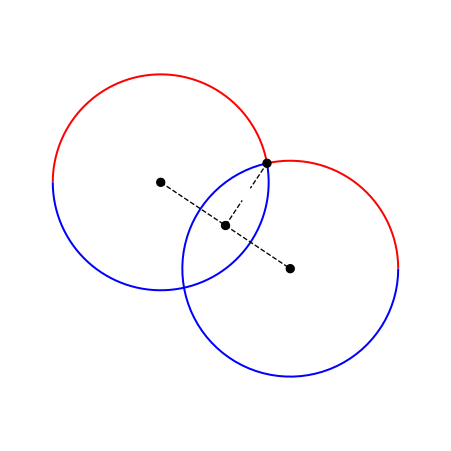
\includegraphics[width=0.45\textwidth]{intersection_two_circles.png} &
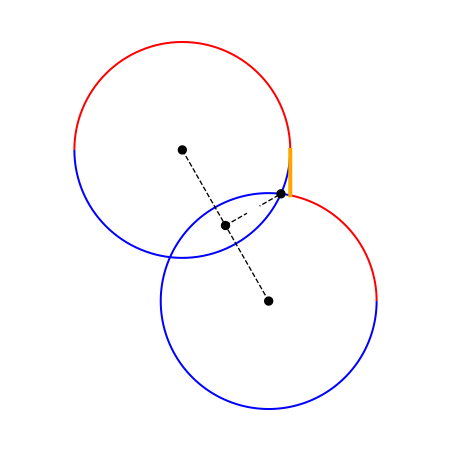
\includegraphics[width=0.45\textwidth]{intersection_two_circles_shadow.png} \\
\textbf{A} & \textbf{B}
\end{tabular}
\caption{Comparison of the upper boundaries of two unit circles. (A) Intersecting
circles with a continuous upper boundary. (B) A discontinuity (in orange)
when one circle overshadows the other.}
\label{fig:two_circles}
\end{figure}

If $x_j + 2 \leq x_i$, the circles do not overlap horizontally. Even the edge case
$x_j + 2 = x_i$ indicates tangential contact, treated here as nonintersecting.

Compute the distance between the centers:
\[
d = \sqrt{(x_i - x_j)^2 + (y_i - y_j)^2}.
\]

If the circles intersect and their centers are not too close (i.e., $\epsilon < d < 2$, where
$\epsilon$ is a small positive number accounting for floating-point precision), we calculate their
upper intersection point $(x_u, y_u)$ as follows:

\begin{itemize}
    \item Compute the midpoint between the centers:
    \[
    \mathbf{p_m} = \frac{1}{2}(\mathbf{c}_j + \mathbf{c}_i).
    \]
    \item Compute the unit vector $\mathbf{p_n}$ perpendicular to the line connecting the centers and
    pointing upright:
    \[
    \mathbf{p_n} = \frac{1}{d}(-(y_i - y_j),\; x_i - x_j).
    \]
    \item Calculate the distance $h$ from the midpoint to the intersection points:
    \[
    h = \sqrt{1 - \left(\frac{d}{2}\right)^2}.
    \]
    \item Compute the upper intersection point:
    \[
    \mathbf{p_u} = \mathbf{p_m} + h \cdot \mathbf{p_n},
    \]
    where $\mathbf{p_u} = (x_u, y_u)$.
\end{itemize}

If $\max(y_j, y_i) < y_u$, then the horizontal transition position is $x_u$.
Otherwise, the horizontal transition position is determined by:
\[
\begin{cases}
x_i - 1, & \text{if } y_j < y_i, \\
x_j + 1, & \text{otherwise.}
\end{cases}
\]

\bibliographystyle{sbc}
\bibliography{referencias}

\end{document}
